\documentclass[]{article}
\usepackage[a4paper, total={15cm,23cm}]{geometry}
\usepackage{fancyhdr}
\usepackage{graphicx}
\usepackage{amsmath}
\usepackage{amssymb}
\usepackage{xcolor}
%opening
\title{PH 222 Activity 7}
\author{Benjamin Bauml}
\date{Winter 2021}
\pagestyle{fancy}
\rhead{PH 222}
\chead{Winter 2021}
\lhead{Activity 7}

%Custom Quotation Command
\newcommand{\excerpt}[1]{\colorbox{lightgray}{\parbox{14.8cm}{#1}} \\}

\begin{document}

\maketitle

\begin{center}
Problems 1, 3, and 4 are borrowed/adapted from Chapter 16 of the \textit{Student Workbook} for \textit{Physics for Scientists and Engineers}.
\end{center}
\section*{Activity 1}%20
\excerpt{
A sinusoidal wave with wavelength 2 m is traveling along the $ x $-axis. At $ t = 0 $ s the wave's phase at $ x = 2 $ m is $ \pi/2 $ rad.
}
\excerpt{
a) Draw a snapshot graph of the wave at $ t = 0 $ s.
}
\begin{center}
	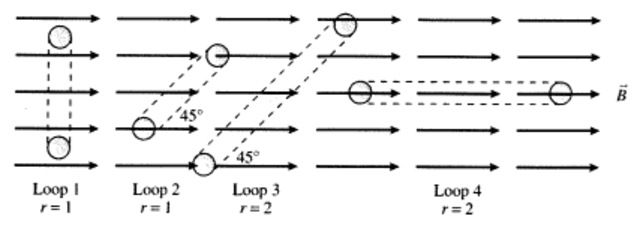
\includegraphics[scale=0.5]{A1}
	%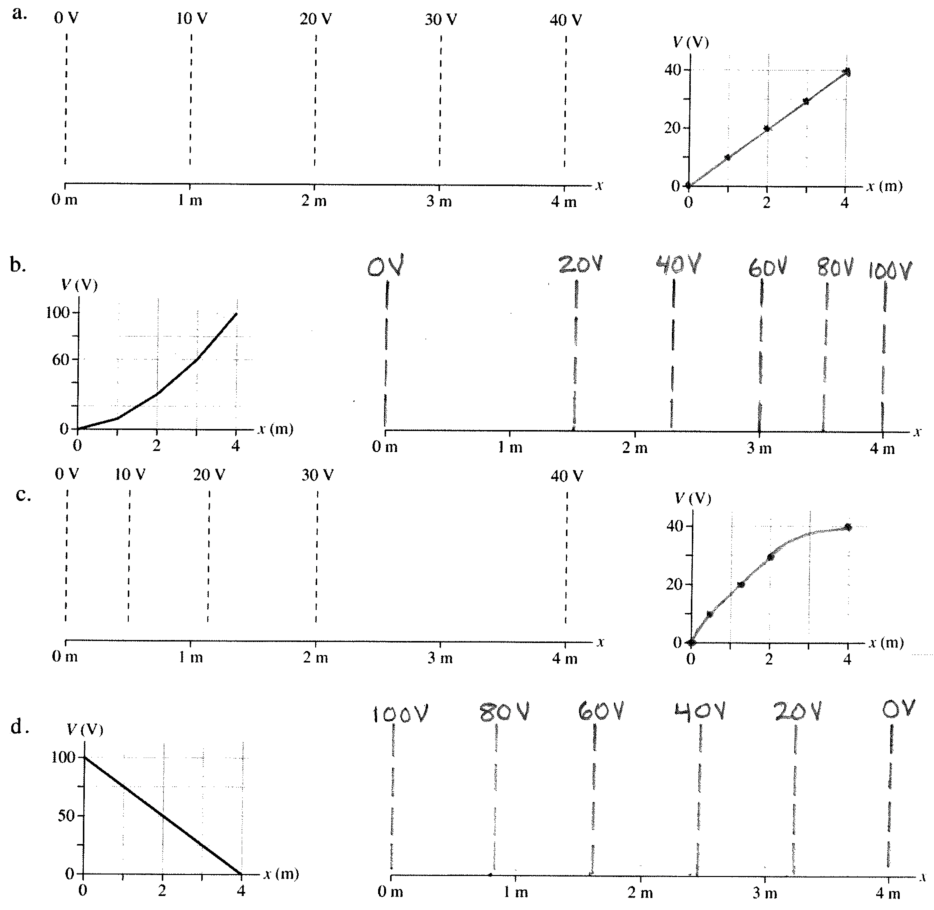
\includegraphics[scale=0.5]{A1Sol}%Solution
\end{center}
% To reveal the solution, delete "\phantom{\parbox{\textwidth}{" from the beginning, and "}}" from the end.
\phantom{\parbox{\textwidth}{
We take the solution of the wave equation to be $ D(x,t) = A\sin(kx\pm\omega t + \phi_{0}) $ (where $ \pm\omega t $ is determined by which way the wave is traveling). The phase of the wave is $ \phi = kx\pm\omega t + \phi_{0} $, so if the phase of the wave at $ x = 2 $ m is $ \phi = \pi/2 $, then the wave ought to peak there. Other peaks occur at even numbered meter marks, as the wavelength $ \lambda = 2 $ m. \\
\indent We can also determine that $ k = \frac{2\pi}{\lambda} = \pi $ m$ ^{-1} $, and therefore at $ x = 2 $ m, $ kx = 2\pi $. Also, $ t = 0 $ s, so the overall phase at this point is
\[
\frac{\pi}{2} = kx + \phi_{0} = 2\pi + \phi_{0},
\]
which means $ \phi_{0} = -\frac{3\pi}{2} $. \\
}}
\excerpt{
b) At $ t = 0 $ s, what is the phase at $ x = 0 $ m? $ x = 1 $ m? $ x = 3 $ m?
}
% To reveal the solution, delete "\phantom{\parbox{\textwidth}{" from the beginning, and "}}" from the end.
\phantom{\parbox{\textwidth}{
In all of these cases, overall phase is
\[
\phi = kx + \phi_{0} = \frac{\pi}{\text{ m}}x - \frac{3\pi}{2} =
\begin{cases}
	- \frac{3\pi}{2}, & \text{if } x = 0 \text{ m}; \\
	- \frac{\pi}{2}, & \text{if } x = 1 \text{ m}; \\
	\frac{3\pi}{2}, & \text{if } x = 3 \text{ m}. \\
\end{cases}
\]
In terms of effective phase between $ 0 $ and $ 2\pi $, these are $ \pi/2 $, $ 3\pi/2 $, and $ 3\pi/2 $, respectively.
}}

\pagebreak
\section*{Activity 2}
\excerpt{
At the top of a post in an open field, a 200 W alarm bell is going off. If the threshold of pain is 130 dB, how close can you get to it without hurting your ears?
}
% To reveal the solution, delete "\phantom{\parbox{\textwidth}{" from the beginning, and "}}" from the end.
\phantom{\parbox{\textwidth}{
The power of this alarm is $ P = 200 $ W, and the sound spreads in a spherical wave, so $ I = \frac{P}{4\pi r^{2}} $. If $ r $ is the distance at which the alarm bell begins to cause pain, then
\[
\begin{split}
	130\text{ dB} & = (10\text{ dB})\log_{10}\left(\frac{I}{I_{0}}\right) \\
	13 & = \log_{10}\left(\frac{I}{I_{0}}\right) \\
	10^{13} & = \frac{I}{I_{0}}.
\end{split}
\]
The threshold of hearing $ I_{0} = 10^{-12} $ W/m$ ^{2} $, so it must be that $ I = 10 $ W/m$ ^{2} $. Solving for $ r $, we find
\[
r = \sqrt{\frac{P}{4\pi I}} = \sqrt{\frac{200\text{ W}}{40\pi\text{ W/m}^{2}}} \approx 1.26\text{ m}.
\]
You could get almost within 1.26 meters of the alarm before it would hurt your ears, but since the alarm is going off for some reason, I recommend you go the other way.
}}

\section*{Activity 3}%32
\excerpt{
You are standing at $ x = 0 $ m, listening to a sound that is emitted at frequency $ f_{0} $. At $ t = 0 $ s, the sound source is at $ x = 20 $ m and moving toward you at a steady $ 10 $ m/s. Draw a graph showing the frequency you hear from $ t = 0 $ s to $ t = 4 $ s. Only the shape of the graph is important, not the numerical values of $ f $.
}
\begin{center}
	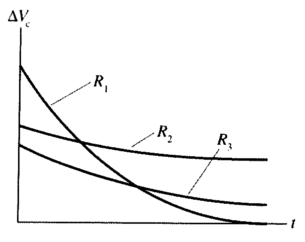
\includegraphics[scale=0.5]{A3}
	%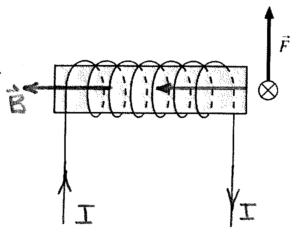
\includegraphics[scale=0.5]{A3Sol}%Solution
\end{center}
% To reveal the solution, delete "\phantom{\parbox{\textwidth}{" from the beginning, and "}}" from the end.
\phantom{\parbox{\textwidth}{
At first, the frequency you percieve is higher, as the source is approaching you. After two seconds, the source has closed the 20 m distance it started at, and passes you. After that, it is moving away at 10 m/s, so the frequency you perceive is lower.
}}

\pagebreak
\section*{Activity 4}%33
\excerpt{
You are standing at $ x = 0 $ m, listening to seven identical sound sources. At $ t = 0 $ s, all seven are at $ x = 343 $ m and moving as shown below. The sound from all seven will reach your ear at $ t = 1 $ s.
}
\begin{center}
	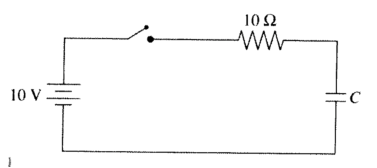
\includegraphics[scale=0.5]{A4}
\end{center}
\excerpt{
Rank in order, from highest to lowest, the seven frequencies $ f_{1} $ to $ f_{7} $ that you hear at $ t = 1 $ s.
}
% To reveal the solution, delete "\phantom{\parbox{\textwidth}{" from the beginning, and "}}" from the end.
\phantom{\parbox{\textwidth}{
Order: $ f_{5}=f_{6}=f_{7} > f_{4} > f_{3}=f_{2}=f_{1} $ \\
Explanation: At a given instant, the sound frequency heard depends on the speed of the source, not its acceleration. Sources 5-7 are moving toward you at the same speed, so all are heard at the same higher frequency. Similarly, sources 1-3 are moving away from you at the same speed, and so will be heard at the same lower frequency.
}}

\section*{Activity 5}
\excerpt{
You are using your phone to generate a 440 Hz tuning pitch (the note A$ _{4} $, or the A above middle C). Your roommate complains that he doesn't like that pitch, and wants it to be 10 Hz higher. If you throw your phone at his head, how fast does it have to be going for him to hear the note he wants? Assume that $ v_{sound} = 343 $ m/s.
}
% To reveal the solution, delete "\phantom{\parbox{\textwidth}{" from the beginning, and "}}" from the end.
\phantom{\parbox{\textwidth}{
The altered frequency due to the Doppler effect is
\[
f' = \frac{f}{1\pm\frac{v_{source}}{v_{sound}}}.
\]
For the frequency to increase, the source must move toward the observer, and the denominator of this fraction must decrease, so the $ \pm $ in the expression sould just be $ - $. We need to solve for $ v_{source} $.
\[
\begin{split}
	1-\frac{v_{source}}{v_{sound}} & = \frac{f}{f'} \\
	v_{source} & = v_{sound}\left(1-\frac{f}{f'}\right) \\
	& = (343\text{ m/s})\left(1-\frac{440\text{ Hz}}{450\text{ Hz}}\right) \\
	& \approx 7.6\text{ m/s}.
\end{split}
\]
This would be some degree of assault, so perhaps you should take anger management classes instead.
}}

\end{document}